\documentclass{beamer}
%\usetheme{Ilmenau}
%\usecolortheme{beaver}

\usepackage[slovak,american]{babel}
\usepackage[utf8]{inputenc}
\usepackage{graphicx}
\usepackage{adjustbox}
 \usepackage{xcolor}
 
 \newsavebox\MBox
\newcommand\Cline[2][red]{{\sbox\MBox{$#2$}%
  \rlap{\usebox\MBox}\color{#1}\rule[-2.2\dp\MBox]{\wd\MBox}{1pt}}}

%\usefonttheme{serif}

%\definecolor{UKOrange}{HTML}{ef9424} %
\definecolor{UKOrange}{HTML}{7a2c18} %
\definecolor{UKBrown}{HTML}{a96d5e} %
\definecolor{UKLight}{HTML}{d8b6ab} %
\definecolor{UKDark}{HTML}{7a4f44}
\definecolor{UKDarker}{HTML}{4d312b} 
\definecolor{UKDarkest}{HTML}{2e1e1a}
\definecolor{UKRed}{HTML}{bf1f1c}

\setbeamertemplate{footline}[frame number]{}
\setbeamertemplate{navigation symbols}{}

%\usecolortheme{beaver}
\setbeamertemplate{itemize item}[square]
\setbeamercolor{itemize item}{fg = UKBrown}
\setbeamercolor{itemize subitem}{fg = UKLight}
\setbeamercolor{enumerate item}{fg = UKDark}

\setbeamercolor{footnote}{fg=UKLight}
\setbeamercolor{footnote mark}{fg=UKLight}
\setbeamerfont{footnote}{size=\tiny}
\renewcommand\footnoterule{}

\usetheme{default}
\beamertemplatenavigationsymbolsempty
\setbeamercolor{title}{fg=white, bg=UKBrown}
\setbeamercolor{frametitle}{fg=white, bg=UKBrown}
\setbeamercolor{block title}{bg=UKBrown, fg= white}
\setbeamercolor{block body}{bg =UKLight, fg = UKDarkest}

\setbeamercolor{block title alerted}{bg=UKOrange, fg= white}
\setbeamercolor{block body alerted}{bg =UKLight, fg = UKDarkest}

% odstrani gulicky
\renewcommand*{\slideentry}[6]{}

\useoutertheme[subsection=false]{miniframes}
\AtBeginSection[]{\subsection{}}

\setbeamercolor{below lower separation line head}{bg=UKDark}
\addtobeamertemplate{headline}{}{%
  \begin{beamercolorbox}[colsep=0.5pt]{below lower separation line head}
  \end{beamercolorbox}
}
%\setbeamercolor*{mini frame}{fg=white,bg=UKRosy}
\setbeamercolor{section in head/foot}{fg=UKLight, bg=UKDark}

\usepackage{etoolbox}
\makeatletter
\preto{\@verbatim}{\topsep=0pt \partopsep=0pt }
\makeatother

%\setbeamertemplate{itemize/enumerate body begin}{\normalsize}
%\setbeamertemplate{itemize/enumerate subbody begin}{\normalsize}




%\newcommand{\codeblock}[2]{ \begin{block}{#1} \begin{verbatim}#2\end{verbatim}\end{block}}

%\defbeamertemplate*{title page}{customized}[1][]
%{
%  \begin{centering}
%    \begin{beamercolorbox}[sep=8pt,center]{title}
%      \usebeamerfont{title}\inserttitle
%    \end{beamercolorbox}
%  \end{centering}
%  \bigskip
%
%\begin{columns}[onlytextwidth,T]
%
%
%  \column{27mm}
%  \includegraphics[width=27mm]{images/logoFMFI.png}
%  
%  \column{\dimexpr\linewidth-54mm-6mm}
%  \centering
%  \vspace{5mm}  
%  \usebeamerfont{author}\insertauthor\par
%  \vspace{5mm}
%  \usebeamerfont{institute}\insertinstitute\par
%
%  \column{27mm}
%  \includegraphics[width=27mm]{images/logoUK.png}  
%\end{columns}
%\centering
%\vspace{7mm}
%  \usebeamerfont{date}\insertdate\par
%}



\newcommand{\e}[1]{$\cdot 10^{#1}$}


\title[1st lab]{AIP - Matbal Fundamentals}
\author[Kocur]{Ing. Viktor Kocur \\{\small viktor.kocur@fmph.uniba.sk}}
\institute{DAI FMFI UK}
\date{24.9.2020}

\begin{document}
\selectlanguage{slovak}


\begin{frame}

  \titlepage

\end{frame}

\section{Matlab Basics}
\begin{frame}
\frametitle{Matlab Environment}

\begin{itemize}
\item Matrix Laboratory of Mathworks
\item Since 1984
\item Original IDE for LINPACK a EISPACK libs without Fortran 
\item Optimized for various computations - especially Linear Algebra
\item Simple and fast implementation of computer vision applications
\end{itemize}
\end{frame}

\subsection{How to seek help}

\begin{frame}
\frametitle{Web resources}

Lab and lecture study materials:
\begin{itemize}
%\item \url{https://www.sccg.sk/~kocur/}
\item \url{https://dai.fmph.uniba.sk/w/Image_Processing_Fundamentals/}
\item \url{https://github.com/kocurvik/edu/}
\end{itemize}


External:
\begin{itemize}
\item \url{https://www.mathworks.com/help/matlab/}
\item \url{https://www.mathworks.com/matlabcentral/answers/}
\item \url{https://stackoverflow.com/}
\end{itemize}
\end{frame}

\begin{frame}
\frametitle{Help in Matlab}
  \begin{block}{How to find help in Matlab}
  \begin{itemize}
    \item help command
    \item lookfor keyword
    \item F1
  \end{itemize}
  \end{block}

  \begin{alertblock}{Exercise}
    Test this for the function/keyword 'edge'
  \end{alertblock}
  
  \begin{block}{Note}
    You can use standard unix commands within Matlab (cd, ls, mkdir, ...)
  \end{block}
\end{frame}

\subsection{Variables and basic operations}

\begin{frame}[fragile]
\frametitle{Scalar variables and arithmetic}

  \begin{block}{Variable assignment}
  \begin{verbatim}
    a = 1
    a = 1;  \end{verbatim}
  \end{block}
  
  \pause
  
  \begin{alertblock}{Named}
    Names are case sensitive! They have to start with a letter and need to have less than 63 characters.
  \end{alertblock}
  
  \pause
  
  \begin{block}{Arithmetic}
  \begin{verbatim}
    a = 1 * 2 + 8/9 - 4^(3/2)
    b = a - 1 + 54*24
    a = b*a  \end{verbatim}
  \end{block}
  
  \pause
  
  \begin{alertblock}{Inf and NaN}
  \begin{verbatim}
    1/0 == Inf
    0/0 == NaN  \end{verbatim}
  \end{alertblock}
\end{frame}

\begin{frame}[fragile]
\frametitle{Mathematics - Matrix multiplication}
  \begin{block}{Definícia}
    $$\mathbb{A} \in \mathbb{R}^{m\times n}, \mathbb{B} \in \mathbb{R}^{n\times l}, \mathbb{C} \in \mathbb{R}^{m\times l}, \mathbb{A} \mathbb{B} = \mathbb{C} \iff$$ \\
    $$\forall i \in \hat{m}, \forall j \in \hat{l}, \mathbb{C}_{i,j} = \sum_{k = 1}^n \mathbb{A}_{i,k} \cdot \mathbb{B}_{k,j}$$
  \end{block}
  
  \begin{alertblock}{Columns vs rows}
   We denote $\mathbb{R}^{\textnormal{num rows} \times \textnormal{num columns}}$
   and $\mathbb{A}_{\textnormal{row}, \textnormal{column}}$
  \end{alertblock}
  
\end{frame}

\begin{frame}[fragile]
\frametitle{Vector variables}
  \begin{block}{Assignment of vector variables}
  \begin{verbatim}
    v = [1 2 3]
    w = [1; 2; 3]  \end{verbatim}
  \end{block}
  
  \pause
  
  \begin{alertblock}{Column vs row vectors}
  \begin{verbatim}
    w*v != v*w
    v+w != v+w' \end{verbatim}
  \end{alertblock}
  
  \pause

  \begin{block}{Generating vectors}
  \begin{verbatim}
    r = start:step:end
    r = linspace(start,end,n)  \end{verbatim}
  \end{block}
\end{frame}

\begin{frame}[fragile]
\frametitle{Matrix variables}
  \begin{block}{Matrix assignment}
  \begin{verbatim}
    A = [1 2 3; 4 5 6]
    B = [v; 2*v - 1]
    C = [w w]  
    D = [A; B]\end{verbatim}
  \end{block}  

\pause

%  \begin{block}{Funkcie na generáciu matíc}
%  \begin{verbatim}
%    zeros(n), zeros(sz), zeros(s1,...,sn)
%    ones(n)
%    eye(n) % Matica identity
%    rand(n) % Náh. matica s rovnomernou dist.
%    randn(n) % Náh. matica s norm. dist.
%    magic(n) % Magická matica  \end{verbatim}
%  \end{block}

  
  \begin{block}{Matrix generation functions}
  \begin{itemize}
    \item zeros(n), zeros(sz), zeros(s1,...,sn)
    \item ones(n)
    \item eye(n) - Identity matrix
    \item rand(n) - Random matrix with uniform distribution
    \item randn(n) - Random matrix with normal distribution
    \item magic(n) - Magic matrix
    \end{itemize}
  \end{block}  
  \end{frame}
  
\begin{frame}
  \frametitle{Array operations}
  \noindent\makebox[\textwidth]{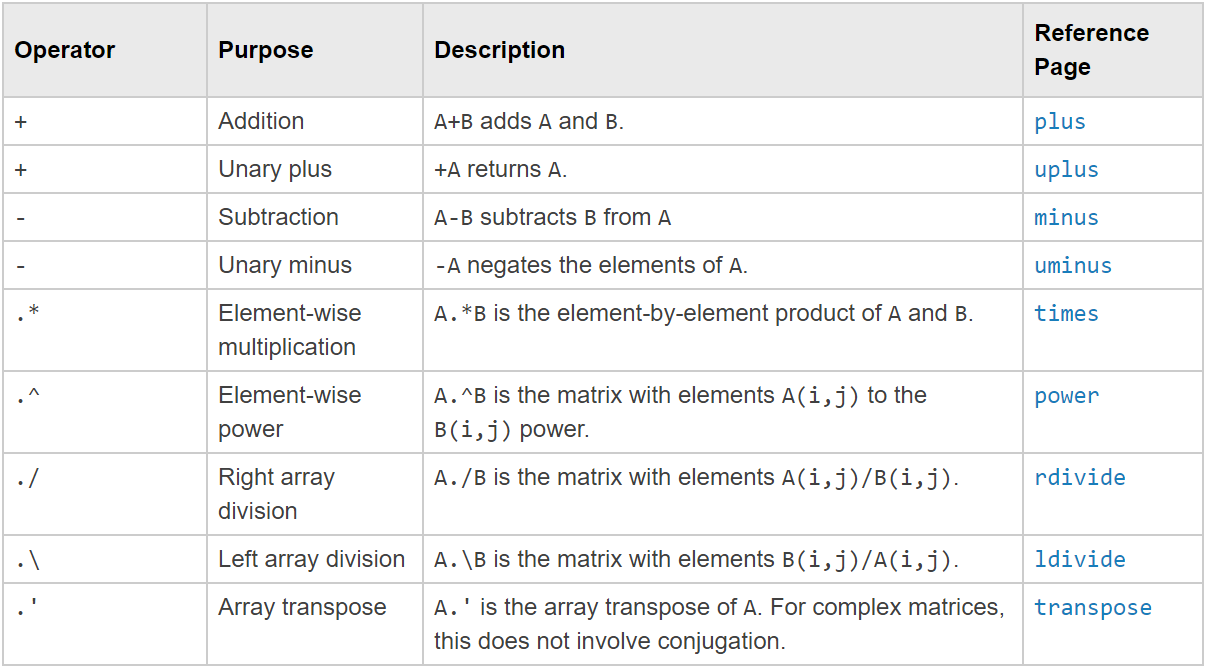
\includegraphics[width=\linewidth]{ArrayOPs.png}}
\end{frame}

\begin{frame}
  \frametitle{Matrix operations}
  \noindent\makebox[\textwidth]{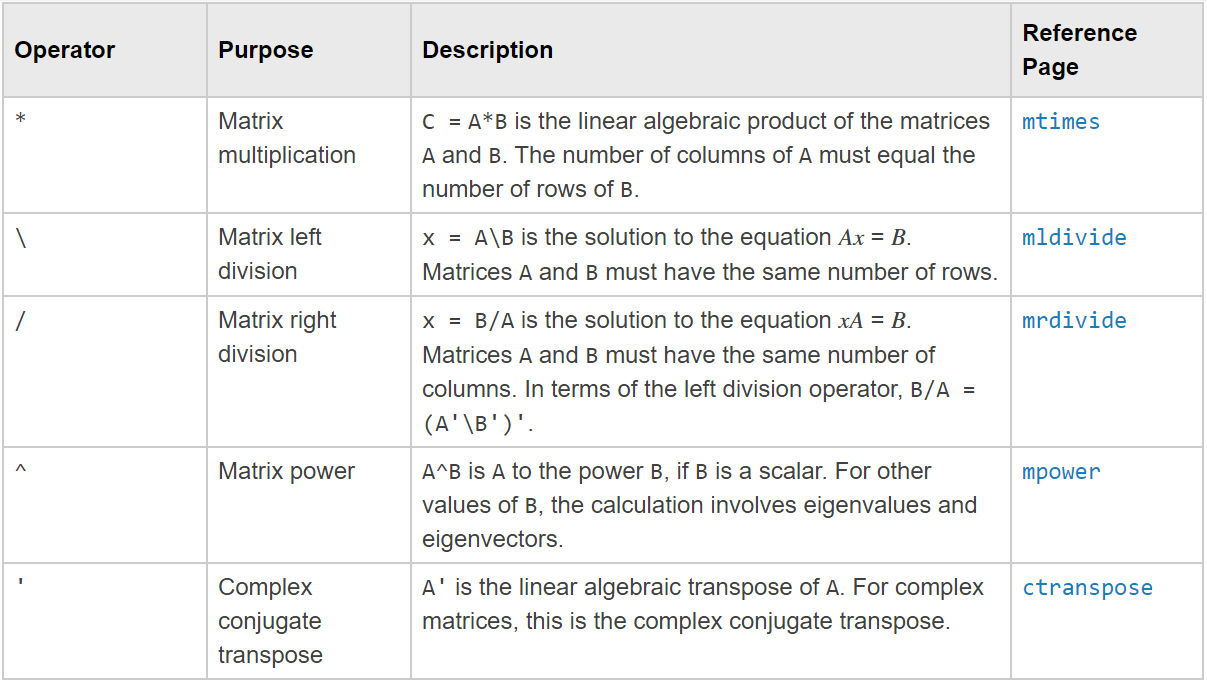
\includegraphics[width=\linewidth]{MatrixOPs.png}}  
  \url{https://www.mathworks.com/help/matlab/matlab_prog/array-vs-matrix-operations.html}
\end{frame}

\begin{frame}[fragile]
  \frametitle{Relation operators}
  \begin{block}{Relation operators - return the logical type}
  \begin{verbatim}
    <, <=, >, >=, ==, ~=\end{verbatim}  
  \end{block}
  
  \pause
  
  \begin{block}{We can compare vectors and matrices}
  \begin{verbatim}
    A = rand(5)
    B = rand(5)
    A > B
    A > 0.5 \end{verbatim}
  \end{block}
\end{frame}

\begin{frame}[fragile]
  \frametitle{Logical operations}
  \begin{block}{Logical functions and operators - return and use the logical type}
  \begin{verbatim}
    and (&), or (|), not (~), xor\end{verbatim}  
  \end{block}
  
  \begin{block}{Short-circuit operators - for scalars only}
  \begin{verbatim}
    &&, ||\end{verbatim}  
  \end{block}
  
  
  \pause
  
  \begin{block}{Reduction to one value}
  \begin{itemize}
    \item any(a) -Returns true if any element is true
    \item all(a) - Returns true if all elements are true
  \end{itemize}
  \end{block}    
\end{frame}


\begin{frame}[fragile]
\frametitle{Matrix operation functions}

%  \begin{lstlisting}
%	flip(A)
%	rot90(A)
%	ones(n),ones(s1,...,sn), ones(sz)
%	eye(n), ...
%	zeros(n), ...
%	rand(n)
%	magic(n)
%	transpose(A), A'
%	.OP - prevedie operaciu postupne pre element po elemente
%	repmat(A,n), repmat(A,s1,...,sn)
%	reshape(A,s1,..,sn), reshape(A,sz)
%	size(A)
%  \end{lstlisting}
  
  \begin{block}{Užitočné funkcie}
  \begin{itemize}
    \item flip(A)
    \item rot90(A)
    \item transpose(A), A' - transpose of matrix
    \item inv(A) - inverse matrix
    \item repmat(A,n) - Matrix with $n \times n$ submatrices A 
    \item reshape(A,s1,..,sn) - Reshapes the matrix
    \item squeeze(A) - Removes 'singleton' dimensions 
    \item size(A) 
    \item numel(A) - Number of elements
  \end{itemize}
  \end{block}
  
  Zoznam funkcií na prácu s maticami a poliami: \\
  \url{https://www.mathworks.com/help/matlab/matrices-and-arrays.html}  
\end{frame}

\begin{frame}[fragile]
\frametitle{Exercise for matrix operations}
  
  \begin{block}{Assignment}
  \centering
    Solve the equation $\mathbb{A}\vec{x} = \vec{b}$ \\
    $\mathbb{A} \in \mathbb{R}^{4\times4}, \mathbb{A}_{i,j} = i\cdot (j + 2)$ \\
    $\vec{b} \in \mathbb{R}^4, \vec{b_i} = i^2$
  \end{block}
  
  \pause
  
  \begin{block}{Example solution}
  \begin{verbatim}
    A = (1:4)'*(3:6)
    b = (1:4).^2
    x = A\b'  \end{verbatim}
  \end{block}  
\end{frame}

\subsection{Indexing}

\begin{frame}[fragile]
\frametitle{Vector indexing}
  \begin{alertblock}{Alert}
    Indices start at 1!
  \end{alertblock}  
    
  \begin{block}{Indexing}
  \begin{verbatim}
    v = [7 8 5 2 4 6 5 2]
    v(2) == 8
    v(4:6) == [2 4 6]
    v(1:2:end) == [7 5 4 5]
    v([3 6 2]) == [5 6 8]\end{verbatim}
  \end{block}
  
\end{frame}

\begin{frame}[fragile]
\frametitle{Writing using index}

  \begin{block}{Writing using index}
  \begin{verbatim}
    v = [7 8 5 2 4 6 5 2]
    v(2) = 4
    v(4:6) = [1 2 3]
    v(1:2:end) = [1 3 5 7]
    v([3 6 2]) = 1
    v(70) = 10000\end{verbatim}
  \end{block}
  
  \pause
  
  \begin{alertblock}{We can write beyond the end of a vector, but we cannot read}
  \begin{verbatim}
    v = [1 2 3]
    v(4) %works
    v(4) = 4 %doesn't work \end{verbatim}
  \end{alertblock}
\end{frame}

\begin{frame}
\frametitle{Maticová indexation}
  \begin{alertblock}{Three options for indexation}
    It is necessary to know the difference between these approaches
    \begin{itemize}
      \item with one index
      \item with a pair (row, col) - generally with an n-tuple
      \item with a logical matrix
    \end{itemize}
  \end{alertblock}
\end{frame}

\begin{frame}[fragile]
\frametitle{Matrix indexation - one index}

  \centering
  When using one index we start at the top left and we first traverse downwards through the column. At the end of the column we move onto the top of the next column.
    
  $$\begin{bmatrix}
       1 & 4 & 7 & 10 \\[0.3em]
       2 & 5 & 8 & 11 \\[0.3em]
       3 & 6 & 9 & 12 \\[0.3em]
     \end{bmatrix} $$
\end{frame}

\begin{frame}[fragile]
\frametitle{Matrix indexation - one index}    
  \begin{block}{Čítanie}
  \begin{verbatim}
    A = magic(5)
    A(4) == 10
    A([4 5 6]) == [10 11 24]
    A([4; 5; 6]) == [10; 11; 24]
    A([10 25; 11 15]) == [18 9; 1 25]
    A(4:4:20) == [10 6 7 8 2]
    A(:) == [17 23 4 10 11 24 5 6 12 ...]\end{verbatim}
  \end{block}
  
\begin{block}{Assignment}
  \begin{verbatim}
    A = magic(5)
    A(4) = 10
    A([4 5 6]) = [10 11 24]
    A([10 25; 11 15]) = [100 200; 300 400]
!!! A([10 25; 11 15]) = [100 200 300 400]\end{verbatim}
  \end{block}
\end{frame}

\begin{frame}[fragile]
\frametitle{Matrix indexation - index pair}    
  \begin{block}{Reading}
  \begin{verbatim}
    A = magic(5)
    A(2,2) == 5
    A(:,2) == [24; 5; 6; 12; 18]
    A(1:2:end,1:3)
    A([3 5],3:5)
    A([5 5 4 2 1],[2 4 5])\end{verbatim}
  \end{block}
  
\begin{block}{Writing}
  \begin{verbatim}
    A = magic(5)
    A(2,2) = 1000
    A(1:2:5,1:end-2) = eye(3)
!!! A(1:2:5,1:3) = [1 2 3 4 5 6 7 8 9]
!!! A([5 5],1) = [1 2]\end{verbatim}
  \end{block}   
\end{frame}

\begin{frame}[fragile]
\frametitle{Matrix indexation  - logical matrix}    
  \begin{block}{Reading and writing}
  \begin{verbatim}
    A = rand(5)
    L = A>0.5    
    A(L)
    A(L) = 0 
    B = magic(5)
    B(A < 0.3 | L) = 50 \end{verbatim}
  \end{block}
  
  \pause
  
  \begin{alertblock}{Beware of dimensions}
    The logical matrix needs to have matching dimensions to what we attempt to index.
  \end{alertblock}   
\end{frame}

\begin{frame}[fragile]
\frametitle{Matrix indexation  - changing the indexation approach}    
  \begin{block}{Funkcie for change}
  \begin{verbatim}
    [r,c] = ind2sub(sz,idx)
     idx  = sub2ind(sz,r,c)
     idx  = find(logicalMatrix)\end{verbatim}
  \end{block}  
  
  \pause
  
\begin{block}{Writing beyond the end of matrix}
  \begin{verbatim}
    A = magic(5)
!!! A(26) = 1  % doesn't work not well defined
    A(6,1) = 1 % works \end{verbatim}
  \end{block}   
\end{frame}

\begin{frame}[fragile]
\frametitle{Indexation exercise 1}
 
  \begin{block}{Assigment}
  Generate a matrix with rand(8). Change all the elements that would be black on a chekerboard to 1. Afterwards change all of the elements smaller than 0.3 to 0.
  \end{block}
  
  \noindent\makebox[\textwidth]{
\includegraphics[width=0.2\linewidth]{chessboard.jpg}}  
  
  \pause
  
  \begin{block}{Example solution:}
  \begin{verbatim}
    R = rand(8)
    R(1:2:7,2:2:8) = 1
    R(2:2:8,1:2:7) = 1
    R(R<0.3) = 0 \end{verbatim}
  \end{block}  
\end{frame}

\begin{frame}[fragile]
\frametitle{Indexation exercise 2}
 
  \begin{block}{Assignment}
  Generate a matrix using magic(8) and create a matrix of shape 8x4 from just the elements that would be on the white tiles in a checkerboard.
  \end{block}
  
  \noindent\makebox[\textwidth]{
\includegraphics[width=0.2\linewidth]{chessboard.jpg}}  
  
  \pause
  
  \begin{block}{Example solution:}
  \begin{verbatim}
    A = magic(8)
    s = [1 0;0 1]
    I = repmat(s,4)
    B = reshape(A(I == 1),[8 4]) \end{verbatim}
  \end{block}  
\end{frame}

\begin{frame}
\frametitle{Mathematical functions}
 
  \begin{block}{Príklady funkcií}
    \begin{itemize}
      \item mod, round, floor, ceil
      \item abs, sgn, exp, log, sin, cos, tan, asin...
      \item min, max
      \item sum, diff, mean, var
    \end{itemize}
  \end{block}
 
  Viac na \url{https://www.mathworks.com/help/matlab/functionlist.html}
  
  \begin{alertblock}{Read the documentations}
  For example the function sum applied to a matrix returns a row vector with sums of values for each column. If we want to add all of the elements of the matrix we need to use sum(sum(A)) or sum(A(:)). Same rule applies for mean, var, min, max, ...
  \end{alertblock}  
\end{frame}

\subsection{Data types}

\begin{frame}[fragile]
\frametitle{Data types}
 
  \begin{block}{Numeric types}
    \begin{itemize}
      \item single, double
      \item int8, int16, int32, int64
      \item uint8, uint16, uint32, uint64
    \end{itemize}
  \end{block}
  
  \pause
  
  \begin{block}{Other types}
  \begin{itemize}
      \item char, string
      \item cell array, map, table, categorical array, struct, logical
      \item date, time, time series, timetable
      \item function handle, handle
  \end{itemize}
  \end{block}
  
  \pause
  
  \begin{block}{Type recognition}
  \begin{verbatim}
    class(a)
    whos a \end{verbatim}
  \end{block}
\end{frame}
  
\begin{frame}[fragile]
\frametitle{Numerical types}   
  
  \begin{block}{Type change}
    \begin{verbatim}
    a = 150
    class(a) == 'double'
    b = uint16(a)
    class(b) == 'uint16'
    cast(int8(-50),'uint8') == 0
    typecast(int8(-50),'uint8') == 206
    typecast(-50,'int16') == [0 0 0 0 0 0 73 192]\end{verbatim}    
  \end{block}  
  
  \pause
  
  \begin{alertblock}{Integer overflow}
    \begin{verbatim}
    uint8(200) + uint8(200) == 255 \end{verbatim}
  \end{alertblock}
  
  \pause
  
  \begin{block}{Displaying numbers}
    \begin{verbatim}
    format long
    format shortEng
\end{verbatim}    
  \end{block}  
\end{frame}

\begin{frame}[fragile]
\frametitle{Other types}   
  
  \begin{block}{Cell array}
    \begin{verbatim}
    c = {45, ones(5), 'hello', [1 2 3]}
    c(1) == {[45]}
    c{1} == 45
    c{3} = 5.24754 \end{verbatim}    
  \end{block}  
  
  \pause
  
  \begin{block}{Struct}
    \begin{verbatim}
    s.a = 1;
    s.b = {'A','B','C'}
    s = 
     struct with fields:
      a: 1
      b: {'A'  'B'  'C'}
    p = struct('fieldName',fieldVal) \end{verbatim}
  \end{block}  
\end{frame}

\section{Scripts and functions}

\subsection{Scripts}

\begin{frame}
\frametitle{Scripts}
  \begin{block}{Scripts}
    We save scripts to separate .m files,
  \end{block}
  
  \begin{block}{Running the script}
  \begin{itemize}
      \item We can call the name of the m-file in the command window provided the script is in path or current folder
      \item Running from the editor - option to debug
  \end{itemize}
  \end{block}
  
  \pause
  
  \begin{alertblock}{Alert!}
    Scripts have access to the variables in the workspace
  \end{alertblock}  
\end{frame}
    
\subsection{Functions}

\begin{frame}
\frametitle{Functions}
  \begin{block}{Functions}
  Functions are saved in a same fashion as scripts. The difference is that functions have inputs and outputs.
  \end{block}
  
  \pause
  
  \begin{block}{Running}
  Functions are called by the FILENAME of the m-files. The file has to be in the current directory or somewhere in PATH.
  \end{block}
  
\end{frame}

\begin{frame}[fragile]
\frametitle{Functions - structure}
  \begin{block}{Functions}
  \begin{verbatim}
    function output = functionName(input)
    % comment - bude sa zobrazovat v helpe
        output = 2*input;
    % tento comment sa uz nezobrazi v helpe
    end \end{verbatim}
  \end{block}
  
\end{frame}

\begin{frame}[fragile]
\frametitle{Functions - structure}
  
  \begin{block}{Multiple inputs and outputs}
  \begin{verbatim}
    function [out1,out2] = functionName(in1,in2)
        out1 = 2*in1;
        out2 = in1*in2;
    end \end{verbatim}
  \end{block}

  \begin{block}{Variable inputs and outputs}
  For variable amount of inputs and outputs we can use special variables nargin (number of inputs) and vararging (array of the inputs) for inputs and nargout for the number of outputs.

  \end{block}
\end{frame}

\begin{frame}[fragile]
\frametitle{Functions - nested a local}
  \begin{block}{Functions}
  \begin{verbatim}
    function parent
        disp('This is the parent function')
        nestedfx
        localfx

        function nestedfx
            disp('This is the nested function')
        end
    end 
    
    function localfx
        disp('This is a local function')
    end\end{verbatim}
  \end{block}
\end{frame}

\begin{frame}
\frametitle{Funkcie}
  \begin{block}{Nested functions}
  Nested functions have access to the variables of the parent function and vice versa. If we use a variable which is not defined in the parent function this variable is then lost after calling the nested function.
  \end{block} 

  \begin{block}{Local functions}
    Local functions do not have access to the variables of the parent function.
  \end{block}  
\end{frame}

\begin{frame}[fragile]
\frametitle{Anonymous functions}
  \begin{block}{Example - essentially a wrapper}
  \begin{verbatim}
    sqr = @(x) x.^2;
    sqr(5) == 25
    
    q = integral(sqr,0,1);
    q = integral(@(x) x.^2,0,1); \end{verbatim}
  \end{block}
\end{frame}

\subsection{Control Flow}

\begin{frame}[fragile]
\frametitle{If}
  \begin{block}{Structure}
  \begin{verbatim}
    if expression
        statements
    elseif expression
        statements
    else
        statements
    end \end{verbatim}
  \end{block}
\end{frame}

\begin{frame}[fragile]
\frametitle{Switch}
  \begin{block}{Structure}
  \begin{verbatim}
    switch switch_expression
        case case_expression
            statements
        case case_expression
            statements
            ...
        otherwise
            statements
    end \end{verbatim}
  \end{block}
\end{frame}

\begin{frame}[fragile]
\frametitle{For cycle}
  \begin{block}{Structure}
  \begin{verbatim}
   for index = values
       statements
   end
   
   for i = 1:n
       	r(i) = ...
   end
   
   for i = [5 0 2 7 5 1]
       	statements
   end \end{verbatim}
  \end{block}
\end{frame}

\begin{frame}[fragile]
\frametitle{While cycle}
  \begin{block}{Structure}
  \begin{verbatim}
    while expression
       statements
    end \end{verbatim}
  \end{block}
  
  \pause
  
  \begin{block}{Ending while a for cycle}
  \begin{itemize}
      \item break - ends the whole cycle
      \item continue - skips to the next iteration
  \end{itemize}
  \end{block}
  
  \pause
  
  \begin{alertblock}{Terminating the program}
    Any script or function can be terminated by pressing Ctrl + C
  \end{alertblock}  
\end{frame}

\begin{frame}
\frametitle{Exercise}
  \begin{block}{Assignment}
  Write a function fib(n), which returns the n-th element of the Fibonacci sequence.
  \end{block}

  \begin{block}{Assignment - hard version}
  Write a function for a linear recurrent sequence linrek(n,$\vec{a}$,$\vec{b}$), which returns the n-th elenent of the sequence defined as $$f_n = \sum_{i = 1}^{dim(\vec{a})} a_i \cdot f_{n-i},$$ with initial values $f_i = b_i$ pre $i \leq dim(\vec{a}) = dim(\vec{b})$.
  \end{block}
\end{frame}  

\begin{frame}[fragile]
\frametitle{Exercise}
    \begin{block}{Example solution:}
  \begin{verbatim}
    function out = fib(n)
        if n <= 0
            out = 0;
        elseif n == 1
            out = 1;
        else
            out = fib(n-1) + fib(n-2)
        end
    end \end{verbatim}
  \end{block}
  \pause  
  \begin{block}{Or:}
  \begin{verbatim}
    function out = fib(n)
        out = round(1.61803398875^(n-1))
    end \end{verbatim}
  \end{block}
\end{frame}  

\begin{frame}[fragile]
    \begin{block}{Hard version solution:}
  \begin{verbatim}
    function rek = linrek(n,a,b)
        if length(b) >= n
            rek = b(n);
        else
            rek = 0;
            for i=1:length(b)
                rek = rek + a(i) * linrek(n-i,a,b);
            end
        end
    end \end{verbatim}
  \end{block}
\end{frame}

\begin{frame}[fragile]
\frametitle{Exercise - no recursion}
  \begin{block}{Solution example:}
  \begin{verbatim}
    function rek = linrekaprox(n,a,b)
        pol = [-1 a];
        r = roots(pol)';
        m = zeros(size(r));
        for i = 1:numel(a)
            m(i) = sum(r(1:i) == r(i)) - 1;
        end
        rowmat = repmat((1:numel(a))',1,numel(a));
        A = (r.^rowmat).*(rowmat.^m);
        k = A\b';
        rek = round(real(((n.^m).*(r.^n))*k));
    end \end{verbatim}
  \end{block}
\end{frame}

\subsection{Profiling}

\begin{frame}[fragile]
\frametitle{Profiling}
  \begin{block}{Tic Toc}
  \begin{verbatim}
    tic
    statements
    toc \end{verbatim}
  \end{block}
  
  \begin{block}{Cputime}
  \begin{verbatim}
    t1= cputime
    statements
    t2 = cputime
    disp(t2 - t1) \end{verbatim}
  \end{block}
\end{frame}

\begin{frame}[fragile]
\frametitle{Matlab optimization compare the runtimes}
  \begin{block}{No allocation}
  \begin{verbatim}
    p = 0;
    for k=1:10000
        p(k) = k/(sin(k)+2)
    end \end{verbatim}
  \end{block}
  
  \begin{block}{With allocation}
  \begin{verbatim}
    p = zeros(1,10000)
    for k=1:10000
        p(k) = k/(sin(k)+2)
    end \end{verbatim}
  \end{block}
  
  \begin{block}{With vector operations}
  \begin{verbatim}
    k = 1:10000
    p = k./(sin(k)+2) \end{verbatim}
  \end{block}
\end{frame}

\section{Working with images}

\subsection{Plot}

\begin{frame}[fragile]
\frametitle{Plot}
  \begin{block}{Simple plot}
  \begin{verbatim}
    x = linspace(0,10,1000);
    plot(x,sin(x)) \end{verbatim}
  \end{block}
  
  \begin{block}{More arguments}
  \begin{verbatim}
    plot(X,Y,LineSpec) 
    plot(X1,Y1,...,Xn,Yn)
    plot(____, Name, Value) \end{verbatim}
  \end{block}
  
   \begin{block}{Linespec - examples}
   \begin{itemize}
    \item Linestyle - -, --, :, -.
    \item Marker - o, +, *, ., x, s, d
    \item Colors - y, m, c, r, g, b, w, k $\rightarrow$ can be combined e.g. r*-
   \end{itemize}
  \end{block}
\end{frame}

\begin{frame}[fragile]
\frametitle{Images}
  \begin{block}{Hold on a hold off}
  \begin{verbatim}
    x = linspace(0,10,1000);    
    plot(x,sin(x))
    hold on
    plot(x,cos(x)) % the second plot is drawn into the first
    hold off 
    plot(x,cos(x)) % this one redraws the whole plot \end{verbatim}
  \end{block}
  
  \pause
  
  \begin{block}{Figure a Axes}
  \begin{verbatim}
    fig1 = figure % generates a figure window
    ax1 = axes % generates axes \end{verbatim}
  \end{block}
  
  \pause
  
  \begin{block}{Where are plots drawn}
  Plots are drawn into the active figure (gcf) and active axes (gca). If you want to draw somewhere else you can use plot(\_\_\_\_,'Parent',ax4)
  \end{block}
\end{frame}

\begin{frame}[fragile]
\frametitle{Subplot}
  \begin{block}{Multiple plots in one}
  \begin{verbatim}
    ax1 = subplot(2,2,1);
    plot(x,sin(x))       
    ax2 = subplot(2,2,2);
    plot(x,cos(x))
    ax3 = subplot(2,2,3);
    ax4 = subplot(2,2,4);
    plot(x,x.^2,'Parent',ax3)
    plot(x,x.^3,'Parent',ax4) \end{verbatim}
  \end{block}
\end{frame}

\begin{frame}
\frametitle{Other plot types}
  
   \begin{block}{Other plot types}
   \begin{itemize}
    \item plot3, loglog, semilogx, semilogy, errorbar
    \item bar, bar3, barh, barh3, histogram, pie, pie3
    \item stem, stairs, scatter
    \item countour, countourf, surf, ezsurf
    \item feather, quiver, compass
   \end{itemize}
  \end{block}
  
  \pause 
  
   \begin{block}{Removing plots}
   \begin{itemize}
    \item cla, clf - clears active axis/figure
    \item close all - closes all figure windows
   \end{itemize}
  \end{block}
\end{frame}

\subsection{Images}

\begin{frame}[fragile]
\frametitle{Reading images}
  
  \begin{block}{Images}
    Download the zip from github kocurvik/edu/PSO/supplementary
  \end{block}
  
  \pause 
  
  \begin{block}{Reading}
  \begin{verbatim}
  rgb = imread('zatisie.jpg');
  whos rgb
  d = im2double(rgb)
  whos d
  bw = imread('zatisie.pgm');
  whos bw \end{verbatim}  
  \end{block}
\end{frame}

\begin{frame}[fragile]
\frametitle{Displaying} 
  \begin{block}{imshow}
  \begin{verbatim}
     imshow(rgb)
     imshow(d)
     imshow(bw)   \end{verbatim}  
  \end{block}
  
  \pause
  
  \begin{block}{image}
  \begin{verbatim}
     image(rgb)
     image(d)
     imagesc(bw)
     colormap(gray)   \end{verbatim}  
  \end{block}
\end{frame}

\begin{frame}[fragile]
\frametitle{Writing} 
  \begin{block}{imwrite}
  \begin{verbatim}
     imwrite(rgb, 'filename.png')
     imwrite(d, 'filename.jpg')
     imwrite(bw, 'filename.png')   \end{verbatim}  
  \end{block}
  
  \begin{alertblock}{Alert!}
  If the image is in uint8, then the values are expected to be in the range 0-255. If the image is in double the range is 0.0 - 1.0. Usually what imshow displays that will get saved using imwrite. For other display options this may not be the case!
  \end{alertblock}
\end{frame}

\begin{frame}[fragile]
\frametitle{Exercise} 
  \begin{block}{Reducing a color channel}
  In the color image of the still (zatisie) reduce the red element of RGB to one fifth. Hint: the array is in shape rows x cols x channels.
  \end{block}
  
  \pause
  
  \begin{block}{Solution}
  \begin{verbatim}
    rgb(:,:,1) = 0.2 * rgb(:,:,1); 
    imshow(rgb)   \end{verbatim}  
  \end{block}
\end{frame}

\begin{frame}[fragile]
\frametitle{Exercise - Hard} 
  \begin{block}{Scale}
  Create a function myimresize(I, s), which returns the image scaled by the values s using the nearest point interpolation.
  \end{block}
  
  \pause
  
  \begin{block}{Solution}
  \begin{verbatim}
function I = myimresize(I, s)
    oldrows = size(I,1);
    oldcols = size(I,2);
    r = round(linspace(1,oldrows,round(s*oldrows)));
    c = round(linspace(1,oldcols,round(s*oldcols)));
    I = I(r,c);        
end  \end{verbatim}  
  \end{block}
\end{frame}

\end{document}